% experiment.tex: Chapter describing the experiment

\chapter{The CMS Experiment}
\label{experiment_chapter}

\section{The Large Hadron Collider}
\label{lhc_section}

\TODO{LHC Graphic of accelerator chain}

The Large Hadron Collider (LHC) is the worlds highest energy and largest
particle accelerator with a maximum design luminosity of 14\TeV and a radius of
2804\meters \cite{bruning2004}. It collides protons on protons. In 2012, when
LHC most recently produced collisions, it had a center of mass energy of 7\TeV;
when it turns back on in 2015 after upgrades it will run at either 13\TeV or
14\TeV.

The LHC is located near Geneva, Switzerland, although parts of the accelerator
(including \pointfive, where the CMS detector is located) are in France.

A number of smaller accelerators are used together in series to accelerate
protons to the energies necessary to be injected into the LHC. The first step
is a linear accelerator, \linactwo, which accelerates protons from rest to to
50\MeV. These protons are then injected into a chain of three circular
accelerators, each injecting into the next. The first of these accelerators is
the Proton Synchrotron Booster (PSB) which accelerates the protons to 1.4\GeV.
The second is the Proton Synchrotron (PS) which accelerates the protons to
26\GeV. The third and final accelerator in the Super Proton Synchrotron (SPS)
which accelerates the protons to 450\GeV and injects directly into the LHC.

Bunches of protons are accelerated using this system and injected into the LHC
to form two, counter-rotating beams. When the desired number of bunches have
been injected into the LHC, the LHC accelerates them to 4\TeV. When the beams
have reached their nominal energy, they are focused and brought into collision
at four different points on the ring where the various experiments (\ALICE,
\ATLAS, \LHCB, and CMS) are located.

The beams are steered around the accelerator ring by a series of
superconducting, dipole magnets. When running at a center of mass energy of
8\TeV, these magnets operate at roughly 7.5\Tesla. There are also quadrapole
and some higher order magnets around the ring used to focus the beams. The
bunches of protons are accelerated by 16 superconducting radio frequency
cavities. These cavities accelerate slower protons while slowing faster ones,
thereby keeping the proton bunches compact in both real and momentum space.
There is room for 2808 bunches in LHC, although in 2012 there were only
\TODO{how many bunches?}.

The LHC is also the highest luminosity collider in the world. The instantaneous
luminosity is given by
\begin{equation}
    \TODO{\luminosity=fn\frac{N^{2}}{\sigma}}
\end{equation}
where $f$ is the frequency of interaction (which is fixed by the LHC's
circumference), $n$ is the number of bunches in a beam, $N$ is the number of
protons per bunch (with the $N^{2}$ coming from the assumption that there are
the same number of protons in the two colliding bunches), and $\sigma$ is the
area profile of the beams. Although a higher luminosity means more particles
are produced and more data can be collected, the maximum luminosity is limited
by several practical factors. The first factor is cost; a higher luminosity
general requires a more expensive machine as the ring is either made larger or
the technology needed to run the machine is made more complex. The second is
the challenge that higher luminosities present to the analyzers. The luminosity
can be increased by increasing the number of protons in a bunch or by squeezing
the bunches more tightly, but eventually the probability of getting multiple
proton-proton interactions per bunch crossing becomes large, leading to a
phenomenon known as pileup. These extra interactions add additional particles
to the detector and can make it difficult to separate interesting events from
uninteresting background. The luminosity can also be increased by increasing
the number of bunches in the machine, but this decreases the time between the
collisions and leads to a phenomenon known as out of time pileup which can also
obscure interesting events. In 2012, the optimal luminosity was achieved by
running with bunches spaced by 50\ns instead of the design nominal bunch
spacing of 25\ns. The decision to use this bunch spacing was driven by
\linactwo which had trouble injecting high population bunches.

\section{The Compact Muon Solenoid}
\label{cms_section}

\TODO{CMS cutaway detector picture \label{cms_cutaway_fig}}

The Compact Muon Solenoid (CMS) is one of two general purpose particle
detectors built on the LHC ring \cite{cms_tdr_1}\cite{cms_tdr_2}. CMS is
designed to detect the very high energy, sub-atomic particles that are produced
in the LHC's proton-proton collisions. CMS is designed to have a high
acceptance and efficiency for these collisions. Here acceptance indicates the
area in both physical space as well as the area in energy and momentum space in
which the detector can detect particles. Efficiency is the probability that a
particle in CMS's acceptance region is properly measured. In order to have a
high acceptance and efficiency, CMS must be both large---to cover a large area
of physical space---and dense---to cover a large area in momentum and energy
space. CMS is \TODO{21\meters in length, 15\meters in diameter, and weighs
14\kilotonne}.

CMS is built as a series of nested, finite cylinders, where each cylinder is a
separate subdetector. The beams enter the detector along the axis of the
cylinder. The collision point is in the center. There are a pair of endcaps on
either side of the cylinder to increase the acceptance of the detector. The
endcaps and central region of the cylinder (call the barrel) overlap to prevent
particles from escaping undetected through the crack. A cutaway of the detector
is shown in \FIG~\ref{cms_cutaway_fig}.

The coordinate system used by CMS is as follows: the origin is the nominal
interaction point at the center of CMS, the \xaxis is defined to point to the
center of the LHC ring, the \yaxis is defined as vertically up, and the \zaxis
points counter-clockwise and tangent to the LHC ring such that it forms a
right-handed coordinate system with the \xaxis and \yaxis. CMS uses a
cylindrical coordinate system with coordinates ($\eta$, $\phi$). The azimuthal
angel $\phi$ is in the \xyplane measured from the \xaxis while $\eta$ is the
pseudorapidity defined by
\begin{equation}
    \eta = -\logn \tan \frac{\theta}{2}
\end{equation}
where $\theta$ is the polar angle with respects to the \zaxis.

\subsection{Inner Tracking System}

\TODO{$\eta$ coverage, electric field, performance}

The inner tracking system, referred to as the tracker, is the subdetector
closest to the interaction point. The tracker's primary purpose is to measure
the charge of particles, the momentum of these same particles, and the location
of interaction vertices---both the primary vertex, the various secondary
proton-proton vertices from pileup, and the vertices of long-lived particles
like b mesons. The tracker consists two types of silicon detectors: silicon
pixels and silicon strips.

\subsubsection{Pixel Tracker}

\begin{figure}[tb]
    \centering
    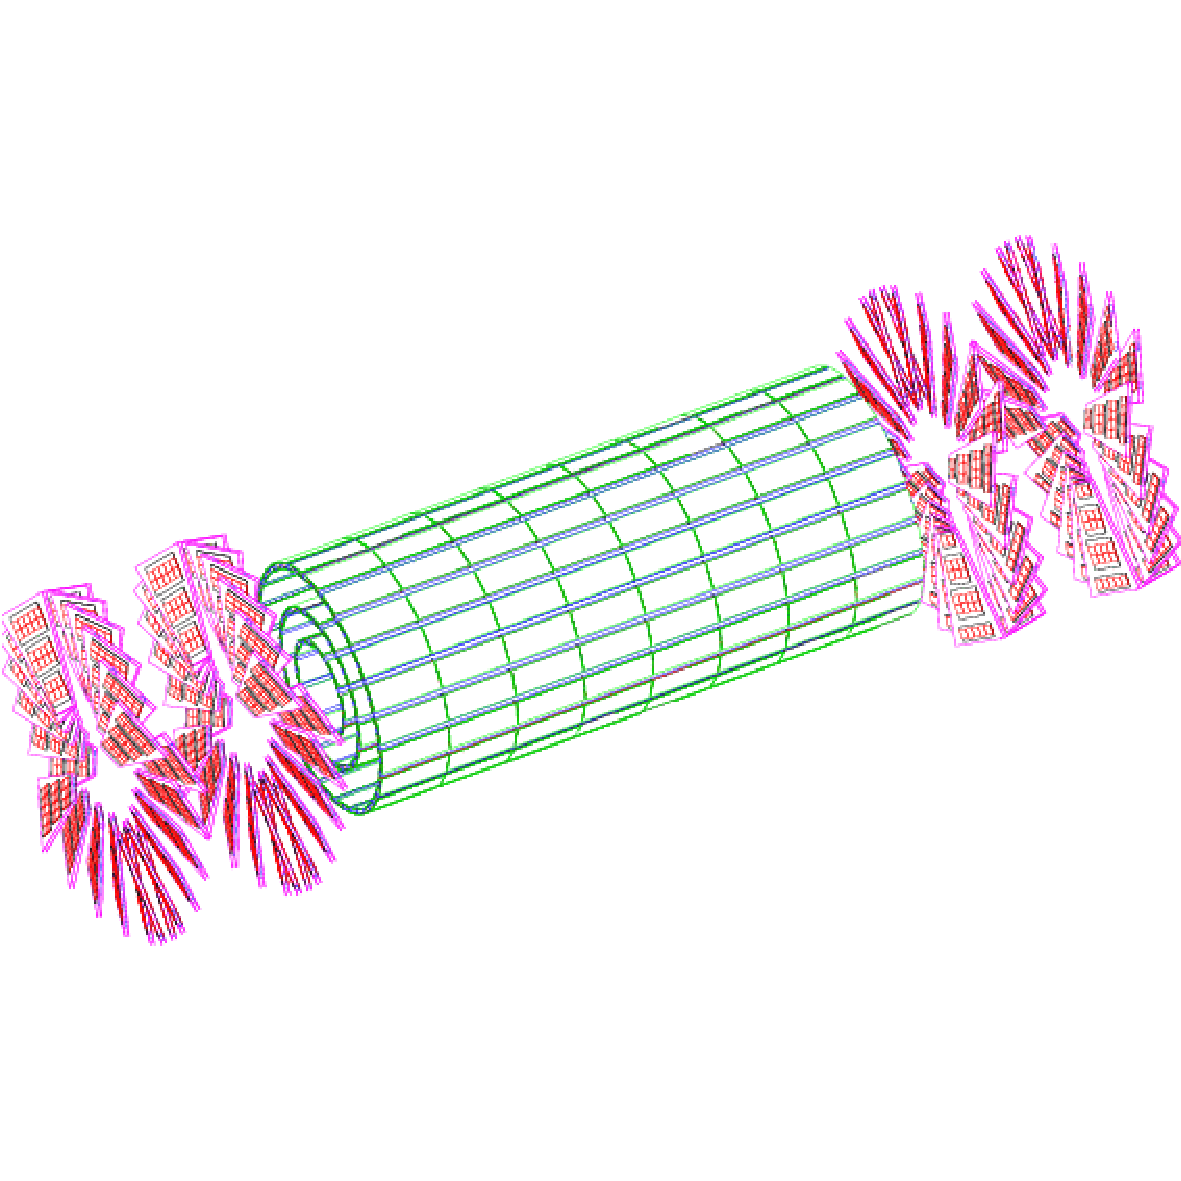
\includegraphics[width=\textwidth]{figures/pixel_layout.pdf}
    \caption{A cross-sectional view of the CMS pixel Tracker.}
    \label{fig:pixel_layout}
\end{figure}

The silicon pixels are used in the region closest to the beam pipe where the
particle flux is the highest and hence the finest granularity is needed. Their
primary purpose is to very accurately locate the primary and secondary vertices
in a collision.

There are three barrel layers of the pixel tracker at radii of of 4.3, 7.3, and
10.2\centimeters, each with a length of 53\centimeters. There are two endcap
annular disks as well placed at $|\coordz|=$ 34.5 and 46.5\centimeters. Each of
these disks has an inner radius of 6\centimeters and an outer radius of
15\centimeters.

Each pixel has an area of $100 \times 150 \micrometers^{2}$, but the resolution
of the tracker is better than that because of charge sharing. If a charged
particle ionizes multiple pixels, then a weighted average of the charges can be
used to get sub-pixel resolution on the location of the hit. In order to
increase the charge sharing, a large Lorentz angle (23\degrees) is used. The
blades which make up the endcap disks are fanned out in a turbine-like geometry
with a rotation of 20\degrees to benefit from the same effect. The layout of
the pixel detector is show in \FIG~\ref{fig:pixel_layout}.

\subsubsection{Strip Tracker}

\begin{figure}[tb]
    \centering
    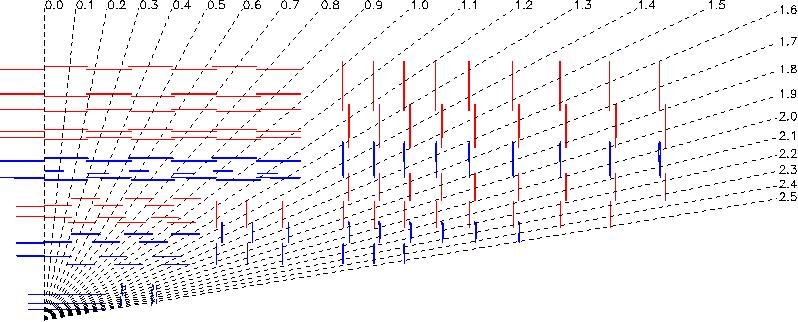
\includegraphics[width=\textwidth]{figures/strip_layout.jpg}
    \caption{A quarter cross-section view of the CMS strip tracker.}
    \label{fig:strip_layout}
\end{figure}

The silicon strips are used further from the beam pipe than the pixels and
cover a much large radius from the beam pipe. The strip tracker has 200 times
the area of the pixel tracker, and so it was not economically feasible to use
the more expensive pixel detectors in this region. The strips' primary purpose
is to measure the momentum and curvature of the charged particles by extending
the tracker's coverage over a larger radius.

Although the strips provide only two points in space to locate a hit (as
compared to three for the pixels), this coarser geometry is adequate because of
the much lower particle flux in this region of the detector. For the momentum,
the location of the hit in the \rphiplane is the most important information,
and so the strips are aligned parallel to the magnetic field. \TODO{Explain
more?}

The strip tracker is itself divided into multiple components. In the barrel
there is the TIB (Tracker Inner Barrel) and the TOB (Tracker Outer Barrel). The
TIB consists of four layers and has coverage up to $|\coordz|<$ 65\centimeters.
The silicon sensors making up the TIB have a strip pitch which varies between
80 to 120\micrometers and have a thickness of 320\micrometers. The first two
layers are constructed with a double layer of modules with a stereo angle of
100\millirads, providing information about the location of the hit in both the
\coordrphi and \rzplane. The TOB consists of six layers and has coverage up to
$|\coordz|<$ 110\centimeters. The TOB has a strip pitch which varies between
120 and 180\micrometers and have a thickness of 500\micrometers. The thicker
sensors are able to be used in this region because the radiation levels are
lower. Having a thicker sensors helps to maintain a high signal-to-noise ratio.
Just like the TIB, the first two layers of the TOB are also build with a double
layer of modules with a stereo angle of 100\millirads.

The ends of the strip tracker consists of the TEC (Tracker Endcap) and the TID
(Tracker Inner Disk). The TEC consists of nine disks in the region
120\centimeters $< |\coordz| <$ 280\centimeters. The TID consists of three
disks in between the end of the TIB and the start of the TEC. The TEC and TID
consist of modules arrayed in rings around the beam line, with the face of each
module pointed towards the interaction point so that they have varying
orientations depending on their distance from the interaction point. The first
two rings of the TID and the first, second, and fifth rings of the TEC are
build with double layer of modules. The modules in the TID and the first three
disks of the TEC have a thickness of 320\micrometers while the rest of the
modules in the TEC have a thickness of 500\micrometers. The strip pitch in the
TID and the first three disks of the TEC have a strip pitch which varies
between 97 and 143\micrometers while the rest of the modules in the TEC have a
strip pitch between 143 and 183\micrometers. The layout of the entire tracker,
including the strip tracker, is shown in \FIG~\ref{fig:strip_layout}.

\subsection{Electromagnetic Calorimeter}

\subsection{Magnet}

The central feature of CMS, both from a design stand point and structurally, is
the large superconducting solenoid magnet. A high strength magnetic field is
required in CMS in order to achieve a momentum resolution of $\Delta \momentum
/ \momentum \approx 10\%$ for muons with $\momentum = 1 \TeVc$. The momentum of
these muons must be measured using their curvature in the tracker and the muon
chambers are they are minimum ionizing particles in the calorimeters.
Additionally, the magnetic field allows the charge of particles to be measured
by the direction in which their tracks curve. The solenoid provides a magnetic
field for all of the components inside the bore of the magnet. The fringing
fields are collected and returns by the iron return yolks which also support
the muon chambers. In this way a field is provided for the muon chambers
without requiring an additional magnet.

The solenoid is 12.9\meters long with an inner bore of 5.9\meters. It generates
a 3.8\tesla field using 2168 turns of conductor which carry 19.5\kiloamps. The
total stored energy is 2.7\gigajoules. The solenoid is encased in aluminum to
help dissipate heat and add strength. This entire assembly is enclosed in a
steel cryostat. The cryostat must be exceptionally strong because it not only
supports the solenoid, but also all of the barrel subdetectors (HCAL, ECAL, and
the tracker) that are mounted within it. The calorimeters and the tracker are
mounted within the solenoid in order minimize the un-instrumented mass---where
particles could lose energy due to interactions---between the calorimeters and
the collision region.
